\usepackage[brazilian,portuges,english]{babel}
% \usepackage{ae} 
\usepackage[utf8x]{inputenc}
\usepackage[T1]{fontenc} 
\usepackage{amsmath}
\usepackage{longtable}
\usepackage{icomma}

%\usepackage[portuges,english]{babel}
\usepackage{copin,mestre} % ,epsfig
\usepackage{times}
\usepackage{multirow}
\usepackage{ucs}
\usepackage{cite}
\usepackage{algorithmic}
\usepackage{algorithm}
\usepackage{bbding}
\usepackage{threeparttable}

%------------------- for doc2latex

%\usepackage{amssymb,amsfonts,textcomp}
%\usepackage{color}
%\usepackage{array}
%\usepackage{supertabular}
%\usepackage{hhline}
\usepackage{hyperref}
\hypersetup{pdftex, colorlinks=false, pdfauthor=Rodrigo Rocha Gomes e Souza,pdftitle=Modelos Computacionais Realistas para Dependências entre Entidades de Software}
%\hypersetup{pdftex, colorlinks=false, linkcolor=blue, citecolor=blue, filecolor=blue, urlcolor=blue, pdftitle=                             , pdfauthor=Rodrigo Souza, pdfsubject=, pdfkeywords=}

%-----------------------------------------------------------------------------------------------------

\usepackage{url}
\usepackage{fancyheadings}
\usepackage{graphicx}
\usepackage{longtable} %tabelas longas, que ultrapassam uma pagina

\usepackage{listings}
\lstset{numbers=left,
stepnumber=1,
firstnumber=1,
%numberstyle=\tiny,
extendedchars=true,
breaklines=true,
frame=tb,
basicstyle=\footnotesize,
stringstyle=\ttfamily,
showstringspaces=false
}
\renewcommand{\lstlistingname}{C\'odigo Fonte}
\renewcommand{\lstlistlistingname}{Lista de C\'odigos Fonte}

\selectlanguage{portuges}
%\selectlanguage{brazilian}
\sloppy

\begin{document}

%%%%%%%%%%%%%%%%%%%%%%%%%%%%%%%%%%%%%%%%%%%%%%%%%%%%%%%%%%%%%%%%%%%%%%%%%%%%%%%%

% Stochastic model: A model that recognizes that there could be a range of possible outcomes for a given set of inputs, and expresses the likelihood of each one happening as a probability. http://wps.pearsoned.co.uk/wps/media/objects/3133/3209133/glossary/glossary.html
% A stochastic model is one that involves probability or randomness. http://www.vertex42.com/ExcelArticles/mc/StochasticModel.html

% Modelos estocásticos? Modelagem e simulação?
\Titulo{Modelos Computacionais Realistas para Dependências entre Entidades de Software}
\Autor{Rodrigo Rocha Gomes e Souza}
% \Data{01/04/2010}
\Data{2010}
\Area{Ciência da Computação}
\Pesquisa{Engenharia de Software}
\Orientadores{Prof. Dr. Dalton Dario Serey Guerrero  
	 (Orientador) \\
	Prof. Dr. Jorge César Abrantes de Figueiredo 
	(Orientador)
	}

\newpage
\cleardoublepage

\PaginadeRosto

\newpage
\cleardoublepage

\vspace*{12cm}
\begin{center}
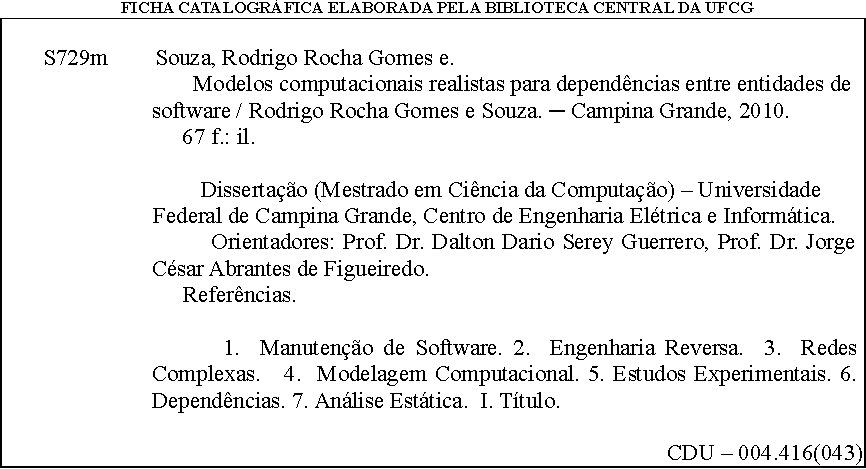
\includegraphics[scale=1]{ficha-catalografica}
\end{center}

\newpage
\cleardoublepage

%%%%%%%%%%%%%%%%%%%%%%%%%%%%%%%%%%%%%%%%%%%%%%%%%%%%%%%%%%%%%%%%%%%%%%%%%%%%%%
\selectlanguage{brazilian}
\begin{resumo} 
% Algoritmos de agrupamento de software agrupam em módulos as entidades do código-fonte de sistemas de software, facilitando a documentação da arquitetura de sistemas. A avaliação empírica desses algoritmos, no entanto, é dificultada pelo fato de existirem poucos sistemas com agrupamentos de referência para serem comparados com os agrupamentos encontrados pelos algoritmos. Neste trabalho é proposta uma abordagem de avaliação usando modelos que produzem grafos que representam sistemas de software organizados em módulos. A abordagem é validada através de um experimento que mostra que os modelos estudados produzem grafos que se assemelham a grafos de dependências estáticas entre entidades de sistemas de software orientados a objetos. Por fim, algoritmos de agrupamento são avaliados através de grafos gerados pelos modelos. Espera-se, com este trabalho, aumentar o conhecimento disponível sobre algoritmos de agrupamento, o que pode contribuir para o seu aperfeiçoamento no futuro.

A análise das dependências entre as entidades do código-fonte de um sistema de software é feita por diversas ferramentas de engenharia reversa com o propósito de revelar informações úteis para a manutenção do software. Existe, no entanto, uma carência de estudos experimentais projetados para avaliar tais ferramentas, em parte devido ao alto custo de se realizar experimentos na área. 

Na área de redes e sistemas distribuídos, o alto custo de experimentação motiva o uso da simulação como meio para avaliar protocolos e algoritmos. Na engenharia reversa, no entanto, simulações são pouco exploradas --- o que se explica parcialmente pela falta de modelos computacionais realistas para dependências entre entidades de código-fonte.

Neste trabalho são apresentados modelos computacionais que geram representações que podem ser interpretadas como dependências entre entidades de código-fonte. Um dos modelos computacionais, chamado BCR+, foi desenvolvido no contexto deste trabalho. Foi desenvolvido também um modelo de classificação que indica, com precisão de 96\%, se uma representação de dependências é realista --- isto é, se ela se assemelha a representações extraídas de sistemas reais. A partir daí foram identificadas configurações de parâmetros para três modelos computacionais (dentre eles, o BCR+) que favorecem a geração de representações realistas.

% Neste trabalho são apresentados três modelos de dependências que podem apoiar a avaliação de ferramentas de engenharia reversa através de simulações controladas. Um dos modelos, chamado BCR+, foi desenvolvido no contexto deste trabalho. Uma avaliação mostrou que, com uma escolha adequada de valores para os parâmetros dos modelos, é possível produzir redes de dependências que se assemelham estruturalmente a redes de dependências extraídas de sistemas de software reais. Ademais, foram derivadas regras que preveem, com 75\% de acurácia, se uma rede gerada com determinada configuração de parâmetros será semelhante a redes extraídas de sistemas de software.

Por fim, é apresentada uma prova de conceito, que demonstra a viabilidade do uso do modelo BCR+ na avaliação de algoritmos usados no contexto de recuperação de arquitetura de software, um ramo da engenharia reversa.

% acurácia de 80%

% <jorge> O resumo carece de números. Acho que já aqui no resumo deve ser mostrado um resumo dos resultados/números. 

% Ao contrário do que ocorre no estudo de redes e sistemas distribuídos, as simulações --- alternativas viáveis aos experimentos quando estes são caros de se realizar --- são pouco exploradas no estudo de ferramentas de engenharia reversa.

% A engenharia reversa, no entanto, carece de modelos realistas para embasar simulações.
\end{resumo}

\newpage
\cleardoublepage

%%%%%%%%%%%%%%%%%%%%%%%%%%%%%%%%%%%%%%%%%%%%%%%%%%%%%%%%%%%%%%%%%%%%%%%%%%%%%%
\selectlanguage{english}
\begin{summary}
% Software clustering algorithms group source code entities into modules, facilitating software architecture documentation. Empirical evaluation of the algorithms, however, is difficult because there are few software systems with reference clusterings for comparison with the clusterings found by algorithms. In this thesis we propose an approach based on models that generate graphs representing software systems with built-in reference clusterings. The approach is validated through an experiment that shows that the models produce graphs resembling the graph of static dependencies between classes in object oriented software systems. Finally, clustering algorithms are evaluated through model generated graphs. It is expected that this study will increase the available knowledge about clustering algorithms, which can contribute to their improvement in the future.
\end{summary}

\selectlanguage{brazilian}

\newpage
\cleardoublepage

%%%%%%%%%%%%%%%%%%%%%%%%%%%%%%%%%%%%%%%%%%%%%%%%%%%%%%%%%%%%%%%%%%%%%%%%%%%%%%
\begin{agradecimentos}
Agradecimentos
\end{agradecimentos}

\clearpage

%%%%%%%%%%%%%%%%%%%%%%%%%%%%%%%%%%%%%%%%%%%%%%%%%%%%%%%%%%%%%%%%%%%%%%%%%%%%%%

%% Definicao do cabecalho: secao do lado esquerdo e numero da pagina do lado direito
\pagestyle{fancy}
\addtolength{\headwidth}{\marginparsep}\addtolength{\headwidth}{\marginparwidth}\headwidth = \textwidth
\renewcommand{\chaptermark}[1]{\markboth{#1}{}}
\renewcommand{\sectionmark}[1]{\markright{\thesection\ #1}}\lhead[\fancyplain{}{\bfseries\thepage}]%
	     {\fancyplain{}{\emph{\rightmark}}}\rhead[\fancyplain{}{\bfseries\leftmark}]%
             {\fancyplain{}{\bfseries\thepage}}\cfoot{}

%%%%%%%%%%%%%%%%%%%%%%%%%%%%%%%%%%%%%%%%%%%%%%%%%%%%%%%%%%%%%%%%%%%%%%%%%%%%%%%%
\selectlanguage{portuges}

\Sumario
% \ListadeSimbolos
\listoffigures
\listoftables
% \lstlistoflistings %lista de codigos fonte - Para inserir a listagem de codigos fonte
\newpage
\cleardoublepage

\Introducao


%%%%%%%%%%%%%%%%%%%%%%%%%%%%%%%%%%%%%%%%%%%%%%%%%%%%%%%%%%%%%%%%%%%%%%%%%%%%%%%%
%
% Hifenizacao - Colocar lista de palavras que nao devem ser separadas e que 
% nao estao no dicionario portugues.
% As palavras do dicionario portugues ja sao separadas corretamente pelo lateX
%
\hyphenation{hardware software}
